\chapter{Аналитический раздел}

В данном разделе приведен обзор функциональности и составляющих статического сервера.

\section{Протоколы TCP и UDP}
Протокол дейтаграмм пользователя UDP не ориентирован на создание соединения, его главное отличие~---~отсутствие гарантии доставки и поддержки упорядоченности передаваемых сообщений до места назначения~\cite{tcp}. Поэтому в приложениях, использующих UDP, разработчики должны реализовывать функции, компенсирующие ненадежность этого протокола: таймауты, повторную передачу, обработку потерянных дейтаграмм и порядковые номера для сопоставления ответов запросам.

Протокол TCP~---~протокол транспортного уровня модели OSI/ISO. Перед началом передачи данных в обязательном порядке устанавливается соединение и использующим его приложениям обеспечивается надежный упорядоченный двухсторонний байтовый поток. Протокол поддерживает отправку и прием подтверждений, обработку таймаутов, повторную передачу, управление потоком и прочие возможности~\cite{tcp}.

Все отправленные данные подлежат обязательному подтверждению встречной стороной, причем формируются подтверждения не для каждого конкретного успешно полученного пакета, а для всех данных от начала посылки до некоторого порядкового номера. Если подтверждение не приходит в течение времени RTO (Retransmission Time Out), то протокол TCP автоматически передает данные повторно и перезапускает таймер вновь. Величина таймера RTO динамически меняется и зависит от времени двухсторонней задержки, определяемой с помощью специальных алгоритмов, типа сети и конкретной реализации протокола.

\section{Протокол HTTP}

HTTP~---~широко распространённый протокол передачи данных, изначально
предназначенный для передачи гипертекстовых документов. Клиенты и серверы взаимодействуют, обмениваясь одиночными сообщениями, а не потоком данных~\cite{http}. 

HTTP-сообщения~---~это формат обмена данными между сервером и клиентом. Есть два типа сообщений:
\begin{enumerate}
	\item запросы, отправляемые клиентом, чтобы инициировать реакцию со стороны сервера;
	\item ответы от сервера.
\end{enumerate}

Сообщения HTTP состоят из текстовой информации в кодировке ASCII, записанной в несколько строк. В HTTP/1.1 и более ранних версиях они пересылались в качестве обычного текста. В HTTP/2 текстовое сообщение разделяется на фреймы, что позволяет выполнить оптимизацию и повысить производительность.

Веб разработчики не создают текстовые сообщения HTTP самостоятельно~---~это делает программа, браузер, прокси или веб-сервер. Они обеспечивают создание HTTP-сообщений через конфигурационные файлы (для прокси и серверов), APIs (для браузеров) или другие интерфейсы.

Так как HTTP это клиент-серверный протокол, соединение всегда устанавливается клиентом. Открыть соединение в HTTP~---~значит установить соединение через соответствующий транспортный протокол, обычно TCP.

В случае с TCP, в качестве порта HTTP-сервера по умолчанию на компьютере используется порт 80, хотя другие также часто используются, например 8000 или 8080. URL загружаемой страницы содержит доменное имя и порт, который можно и не указывать, если он соответствует порту по умолчанию.

\section{Сокеты}

Под сокетом понимают абстракцию конечной точки соединения. Сокеты~---~универсальное средство взаимодействия параллельных процессов, применяемое как на локальной машине, так и в распределенной системе~\cite{ryaznu}.

Сокеты создаются системным вызовом \texttt{socket} со следующими параметрами.

\begin{enumerate}[label=\arabic*)]
	\item Family/Domain~---~домен соединения: Некоторые значения для домена:
	\begin{itemize}[label=---]
		\item AF\_UNIX, AF\_LOCAL~---~локальное соединение;
		\item AF\_INET~---~протокол IPv4;
		\item AF\_INET6~---~протокол IPv6;
		\item AF\_UNSPEC~---~неопределенный;
		\item AF\_NETLINK~---~используется для взаимодействия с ядром.
	\end{itemize}
	\item Type~---~задает семантику коммуникации. Некоторые типы: 
	\begin{itemize}[label=---]
		\item SOCK\_STREAM~---~определяет ориентированное на потоки, надежное, упорядоченное, полудуплексное соединение между двумя сокетами.
		\item SOCK\_DGRAM~---~определяет ненадежную службу datagram без установления логического соединения, где пакеты могут передаваться без сохранения порядка.
		\item SOCK\_RAW~---~обеспечивает доступ к низкоуровневому сетевому протоколу.
	\end{itemize}
	\item Protocol~---~задает конкретный протокол, который работает с сокетом.
	\begin{itemize}[label=---]
		\item IPPPROTO\_TCP (по умолчанию для SOCK\_STREAM).
		\item IPPPROTO\_UDP (по умолчанию для SOCK\_DGRAM).
	\end{itemize}
\end{enumerate}

Взаимодействие на сокетах осуществляется по модели <<клиент-сервер>>: сервер предоставляет ресурсы и службы одному или нескольким клиентам, которые обращаются к серверу за обслуживанием. Схема взаимодействия представлена на рисунке~\ref{img:sock}.

 \begin{table}[H]
	\centering
	\begin{tabular}{p{1\linewidth}}
		\centering
		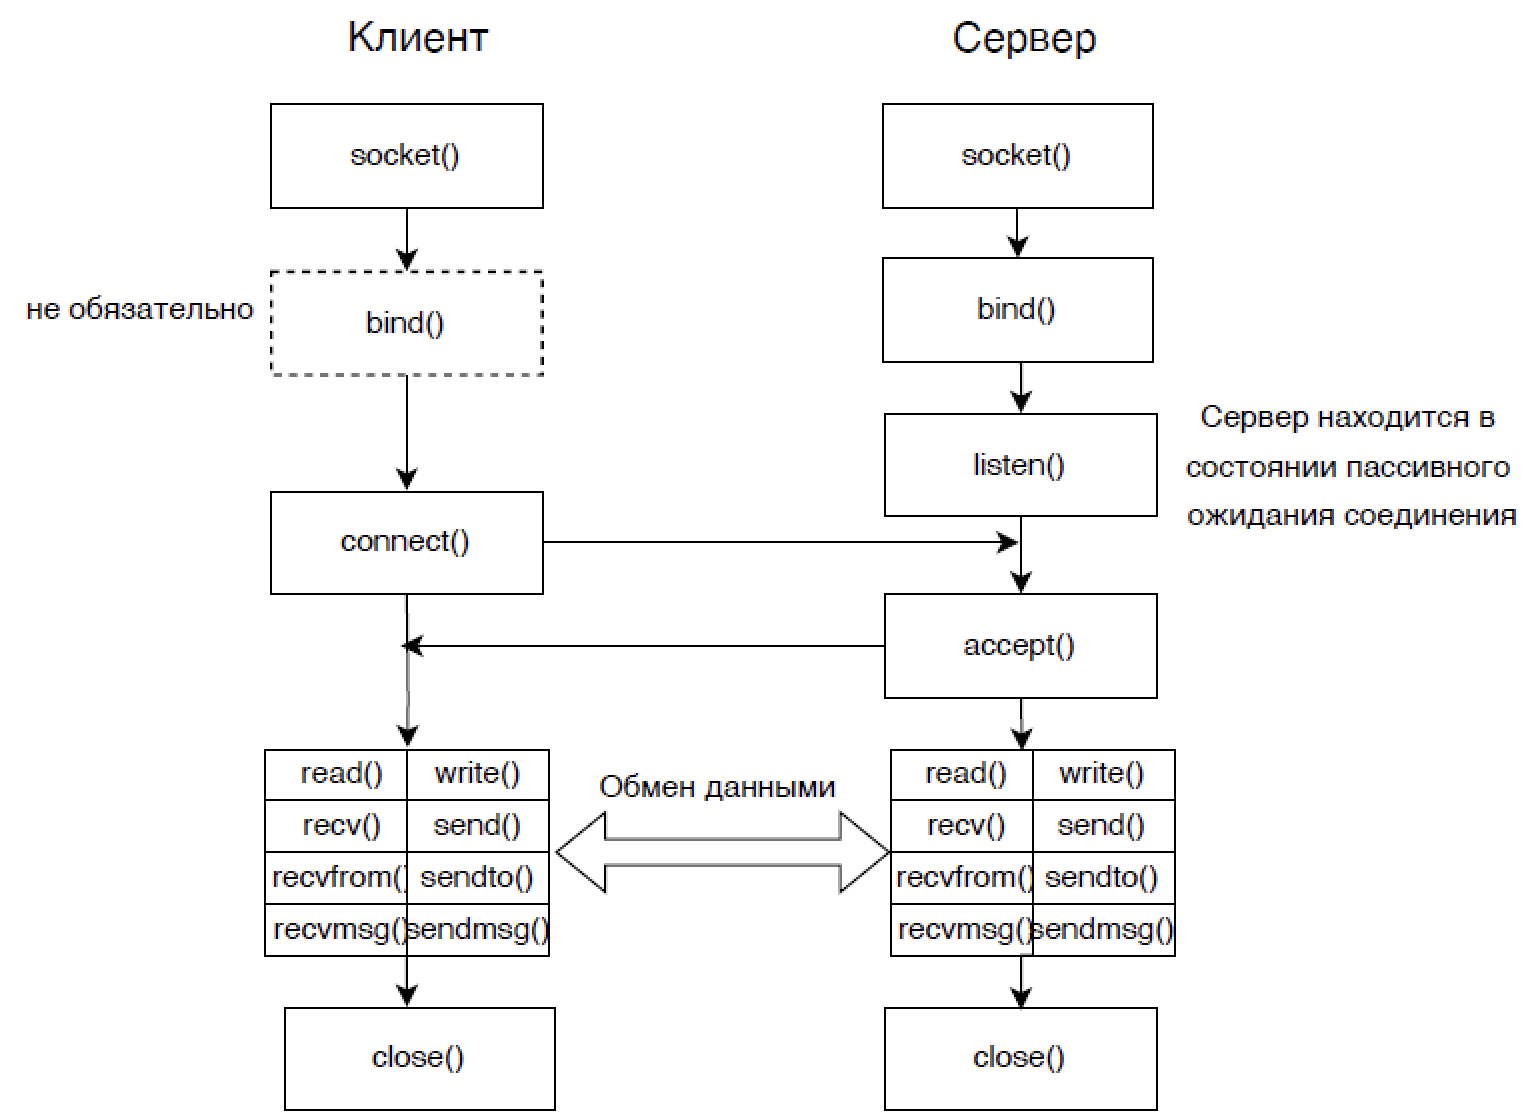
\includegraphics[width=1.0\linewidth]{assets/sock.png}
		\captionof{figure}{Схема взаимодействия на сокетах по модели <<клиент-сервер>>}
		\label{img:sock}
	\end{tabular}
\end{table}

\section{Мультиплексирование}
Для уменьшения времени блокировки сервера на ожидании соединения используется мультиплексирование, т.~к. время установления соединения с первым готовым к взаимодействию меньше, чем с каждым конкретным клиентом в определенной последовательности. Мультиплексор опрашивает соединения. Первое готовое соединение фиксируется ядром. Мультиплексирование является менее затратным вариантом многопоточности. Для мультиплексирования ОС предоставляет системные вызовы, с помощью которых можно обратиться к одному из доступных мультиплексоров. Существующие мультиплексоры:  select, poll, pselect, dev/poll, epoll~\cite{ryaznu}.

На рисунке~\ref{img:sock2} представлена схема мультиплексирования.

 \begin{table}[H]
	\centering
	\begin{tabular}{p{1\linewidth}}
		\centering
		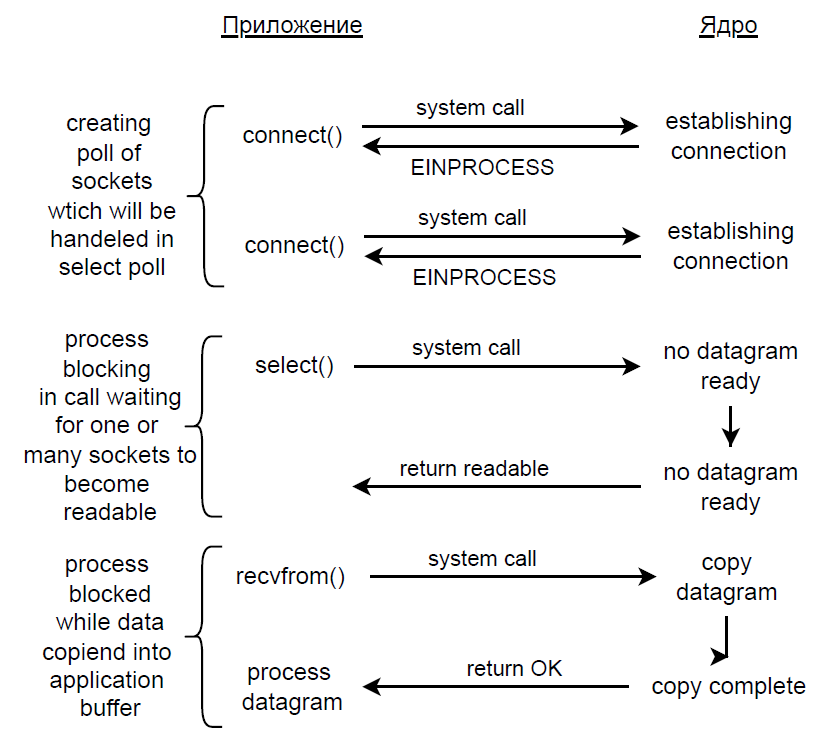
\includegraphics[width=1.0\linewidth]{assets/sock2.png}
		\captionof{figure}{Схема мультиплексирования}
		\label{img:sock2}
	\end{tabular}
\end{table}

\section{Пул потоков}

Пул потоков~---~это фиксированный набор потоков, одновременно выполняющих независимые друг от друга задачи, помещенные в некоторый массив. Массив задач обычно представляется в виде очереди~\cite{ryazanov}.

Перед поступлением заявок в очередь создаются все потоки, которые могут принимать участие в обработке, и переводятся в режим ожидания. Вновь прибывшую задачу достает любой свободный поток из пула и начинает ее выполнять. Закончив обработку, поток возвращается в режим ожидания.

Данный подход позволяет повысить производительность программы, так как избавляет от необходимости в процессе обработки заявок из очереди создавать новые потоки, что было бы трудоемко для ОС.